\section{Latex Examples}

\subsection{Headings}
Sections, sub-sections and sub-sub-sections allow different levels of headings. 
This can be done via the \verb|\section|, \verb|\subsection|, and \verb|\subsubsection| command respectively.
Try to avoid more than 3 levels of headings in your paper!


\subsection{Include files}
If sections are split in several .tex files they can be included via the  \verb|\input | command respectively.
For example:  \verb|\section{Introduction}
\label{sec:introduction}


\lipsum[1-3] \cite{Turing1936}
\begin{figure}[h!]
\centering
  \includegraphics[width=0.8\linewidth]{figures/science_park.jpg}
  \caption{A boat.}
  \label{fig:boat1}
\end{figure}
\lipsum[4-6] | adds the introduction.tex file.  \verb|\input{chapters/chapter1}| would add the chapter1.tex file from the chapters folder. 


\subsubsection{A sub-subsection}

\subsection{Items and Enumerations}
 The environment \verb|\itemize| allows to create a lists whereas the environment \verb|\enumerate| creates a numbered list. Both environments are created via the \verb|\begin{itemize}| and \verb|\end{itemize}| or  \verb|\begin{enumerate}| and \verb|\end{enumerate}| commands.\\
 
 An unordered list:
\begin{itemize}
  \item An Item
  \item Another Item
  \item Yet another Item
\end{itemize}

 An ordered list:
\begin{enumerate}
  \item One
  \item Two
  \item Three
\end{enumerate}

\subsection{Citations}

Latex uses the BibTEX reference management software which allows to cite references using the \verb|\cite| command.
For example~\cite{Turing1936}.


\subsection{Referencing Sections, Figures, and Tables}

References to different items can be created via the  \verb|\ref|.
The items need to be labeled with the \verb|\label| command.

For example, a section labeled with  \verb|\label{sec:introduction}| can be referenced with\newline \verb|\ref{sec:introduction}|. This generates the respective number: ``In section~\ref{sec:introduction} \ldots''\\

\bigskip
We provide a couple of custom commands to make it easier to reference tables, figures and sections that automatically adds the section, table or figure prefix: 

\begin{itemize}
    \item \verb|\citesec|:    ``In~\citesec{introduction} \ldots''
    \item \verb|\citefig|:    ``In~\citefig{sample-fig} \ldots''
    \item \verb|\citetable| : ``In~\citetable{example} \ldots''

\end{itemize}



\subsection{Figures}

An image is added to a document via the \verb|\includegraphics| for jpg, png, or pdf images  or with \verb|\includesvg| for vector images ans shown in \citefig{sample-fig}

\begin{figure}[h!]
\centering
  %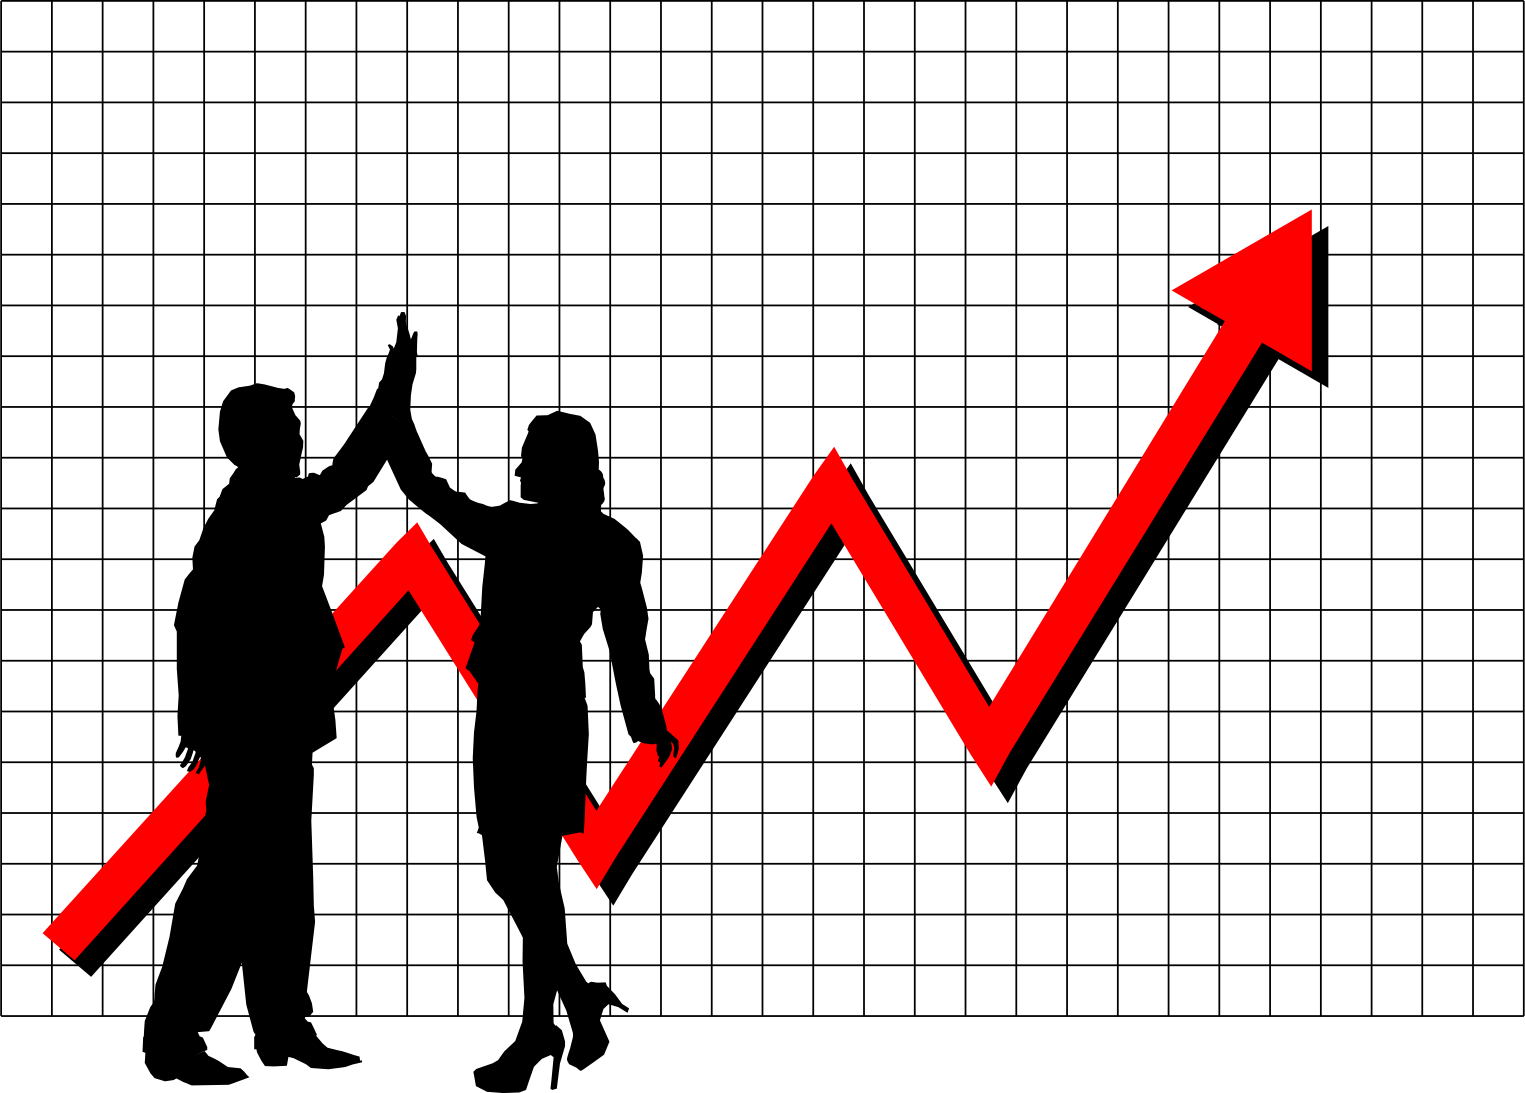
\includegraphics[width=0.8\linewidth]{figures/sample-figure.png}
   \includesvg[width=0.5\linewidth]{figures/sample-figure.svg}
  \caption{A sample svg image}
  \label{fig:sample-fig}
\end{figure}


\subsection{Tables}



A table in \LaTeX\ is created by using a \verb|tabular| environment or any of its extensions, e.g., \verb|tabularx|.
\citetable{example} shows an example of a simple table.

\begin{table}[th!]
\centering
\begin{tabular}{p{4cm}r}
\toprule
Category                & Wind	Speed (Mph)             \\ \midrule
1                       & 25                            \\
2                       & 25                            \\
3                       & 25                            \\ \midrule
4                       & 25                            \\
5                       & \textgreater{}=155           \\ \bottomrule
\end{tabular}
 \caption{The caption of the table}\label{tab:example}
\end{table}

